\section{Hardware Design} \label{sec:hardware}

\subsection{Antenna and Low Noise Amplifier}
The first major hardware improvement over STARE2 is the transition to a new, higher performance low noise amplifier (LNA)~\cite{weinrebLowNoiseAmplifier2021a} developed at Caltech for the DSA-110~\cite{raviDSA110OverviewFirst2023}.
The new amplifier has a noise temperature of $7\,\text{K}$, versus the previous amplifier's noise temperature of $\approx30\,\text{K}$, dramatically improving our system noise temperature and sensitivity.
The LNA achieves record-breaking noise at ambient temperature via the use of an exceptional low noise transistor from Diramics and a low loss suspended stripline input matching network.

For the antenna, we use an improved version of the same ``cake pan'' antenna from STARE2, also designed for the DSA-110.
This is a waveguide horn antenna with cake pans forming axial corrugations, enhancing the beam pattern.
The antenna's full-width half-maximum (FWHM) is estimated to be $70\degree\pm5\degree$ at $1.4\,\text{GHz}$ with very little variation across our band of 1280 to 1530 MHz.
We verify the estimation of the beam width in \autoref{sec:beam_model} by fitting HI intensity data.
As this is an all-sky instrument, the large beam width trades sensitivity for field of view, matching our science goals.

\subsection{Frontend Module}

\begin{figure}[ht!]%
    \centering
    \parbox{.4\textwidth}{
        \centering
        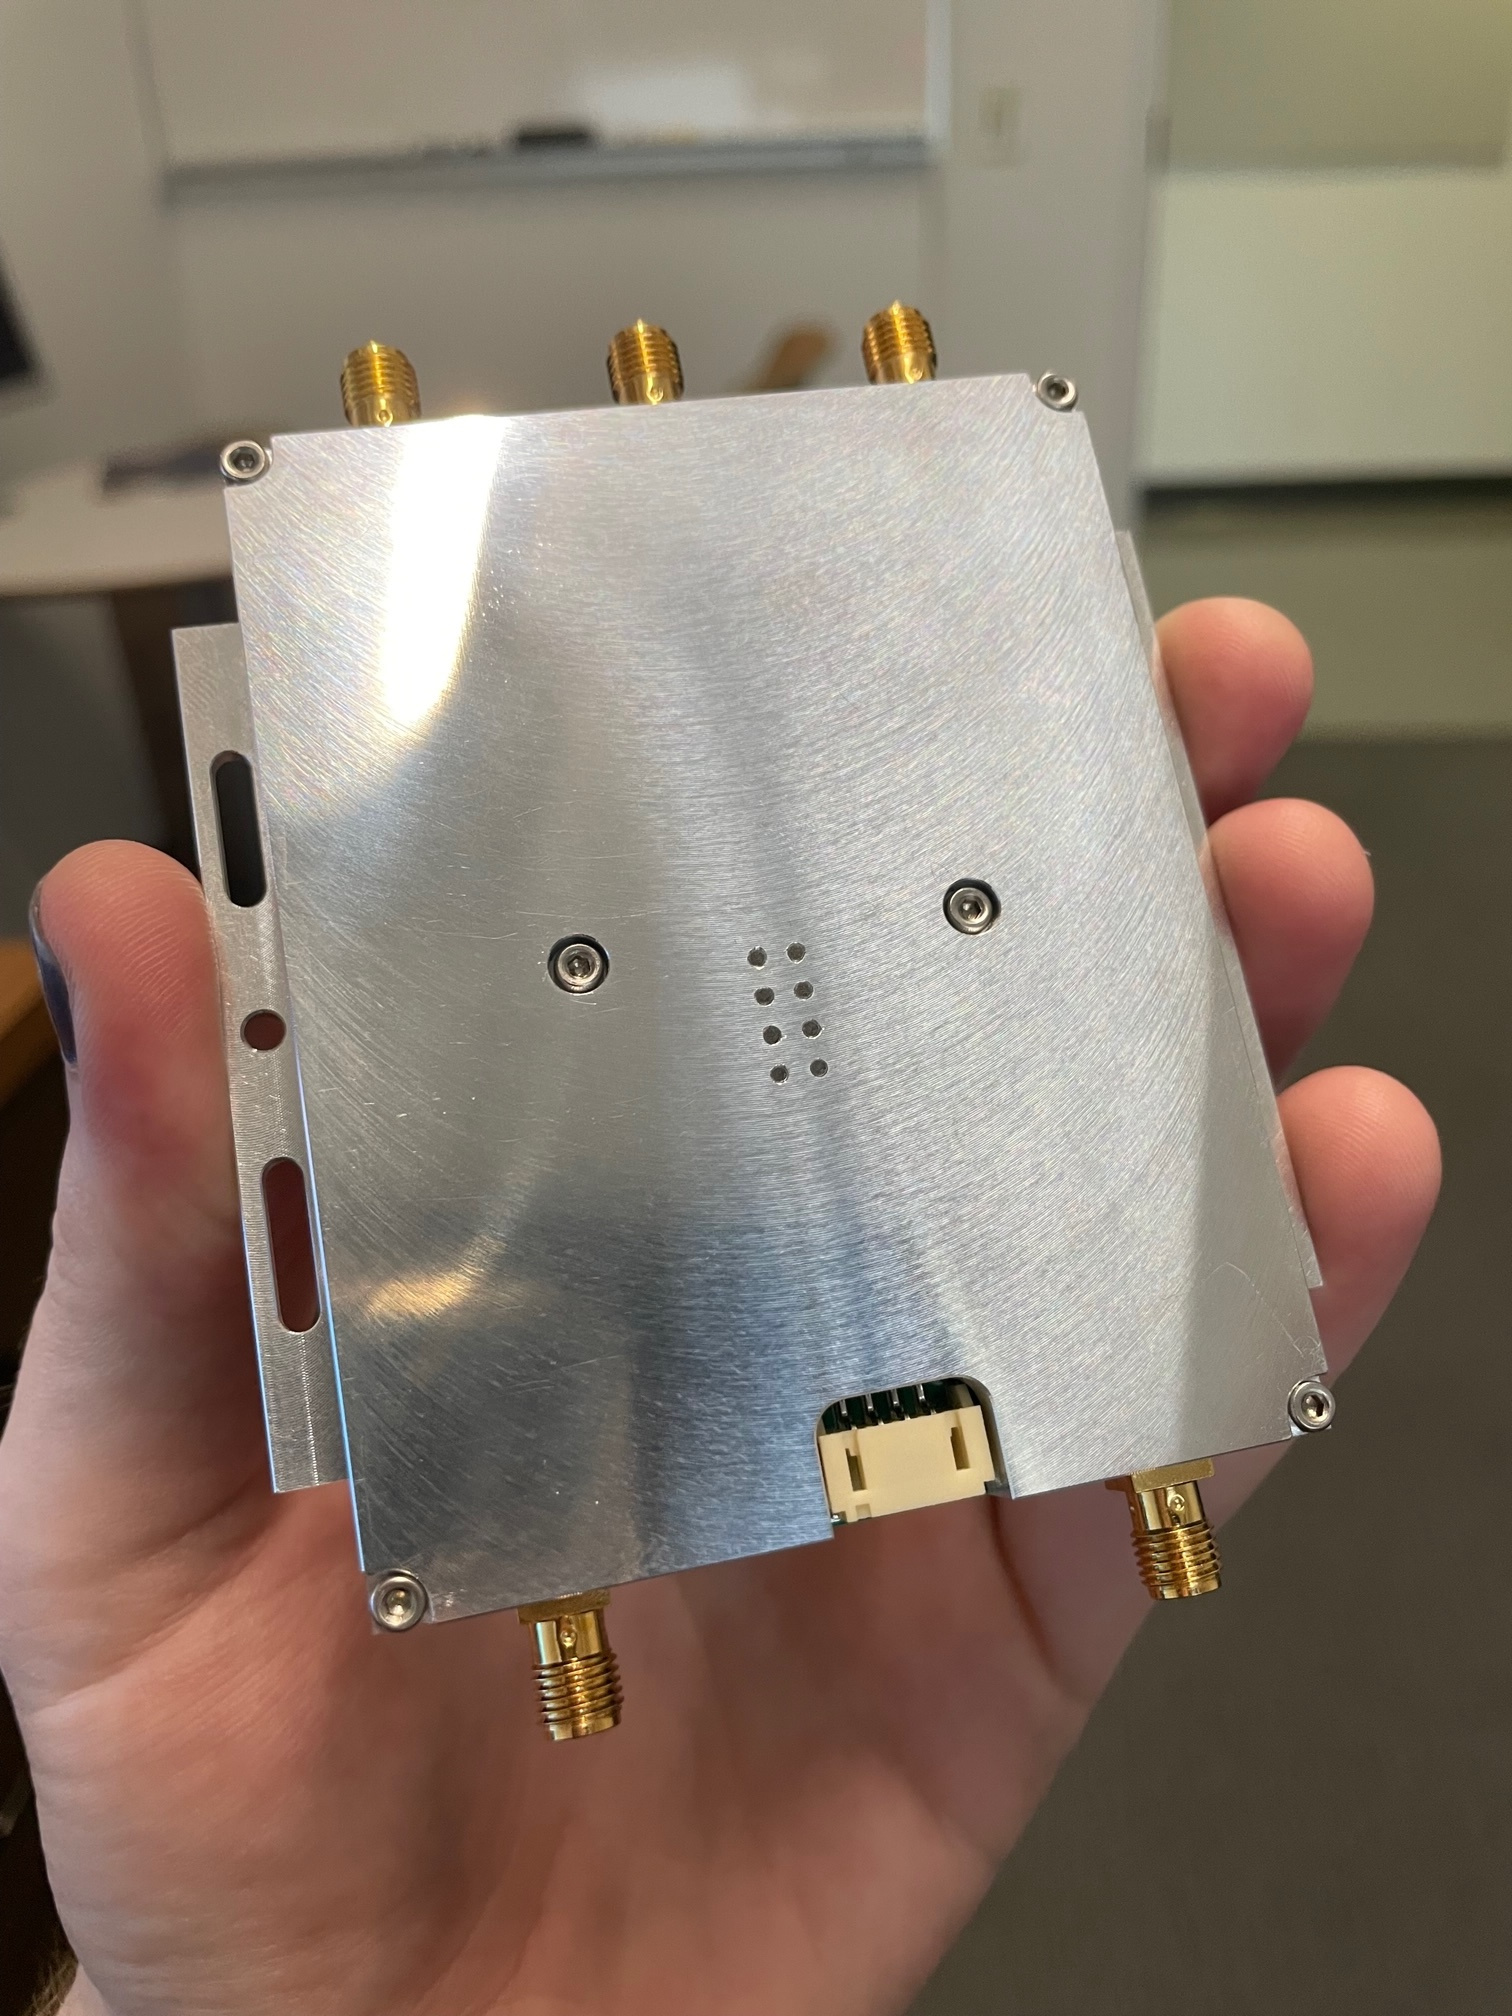
\includegraphics[width=\linewidth]{figures/FEM.jpg}
    }%
    \qquad
    \parbox{.4\textwidth}{
        \centering
        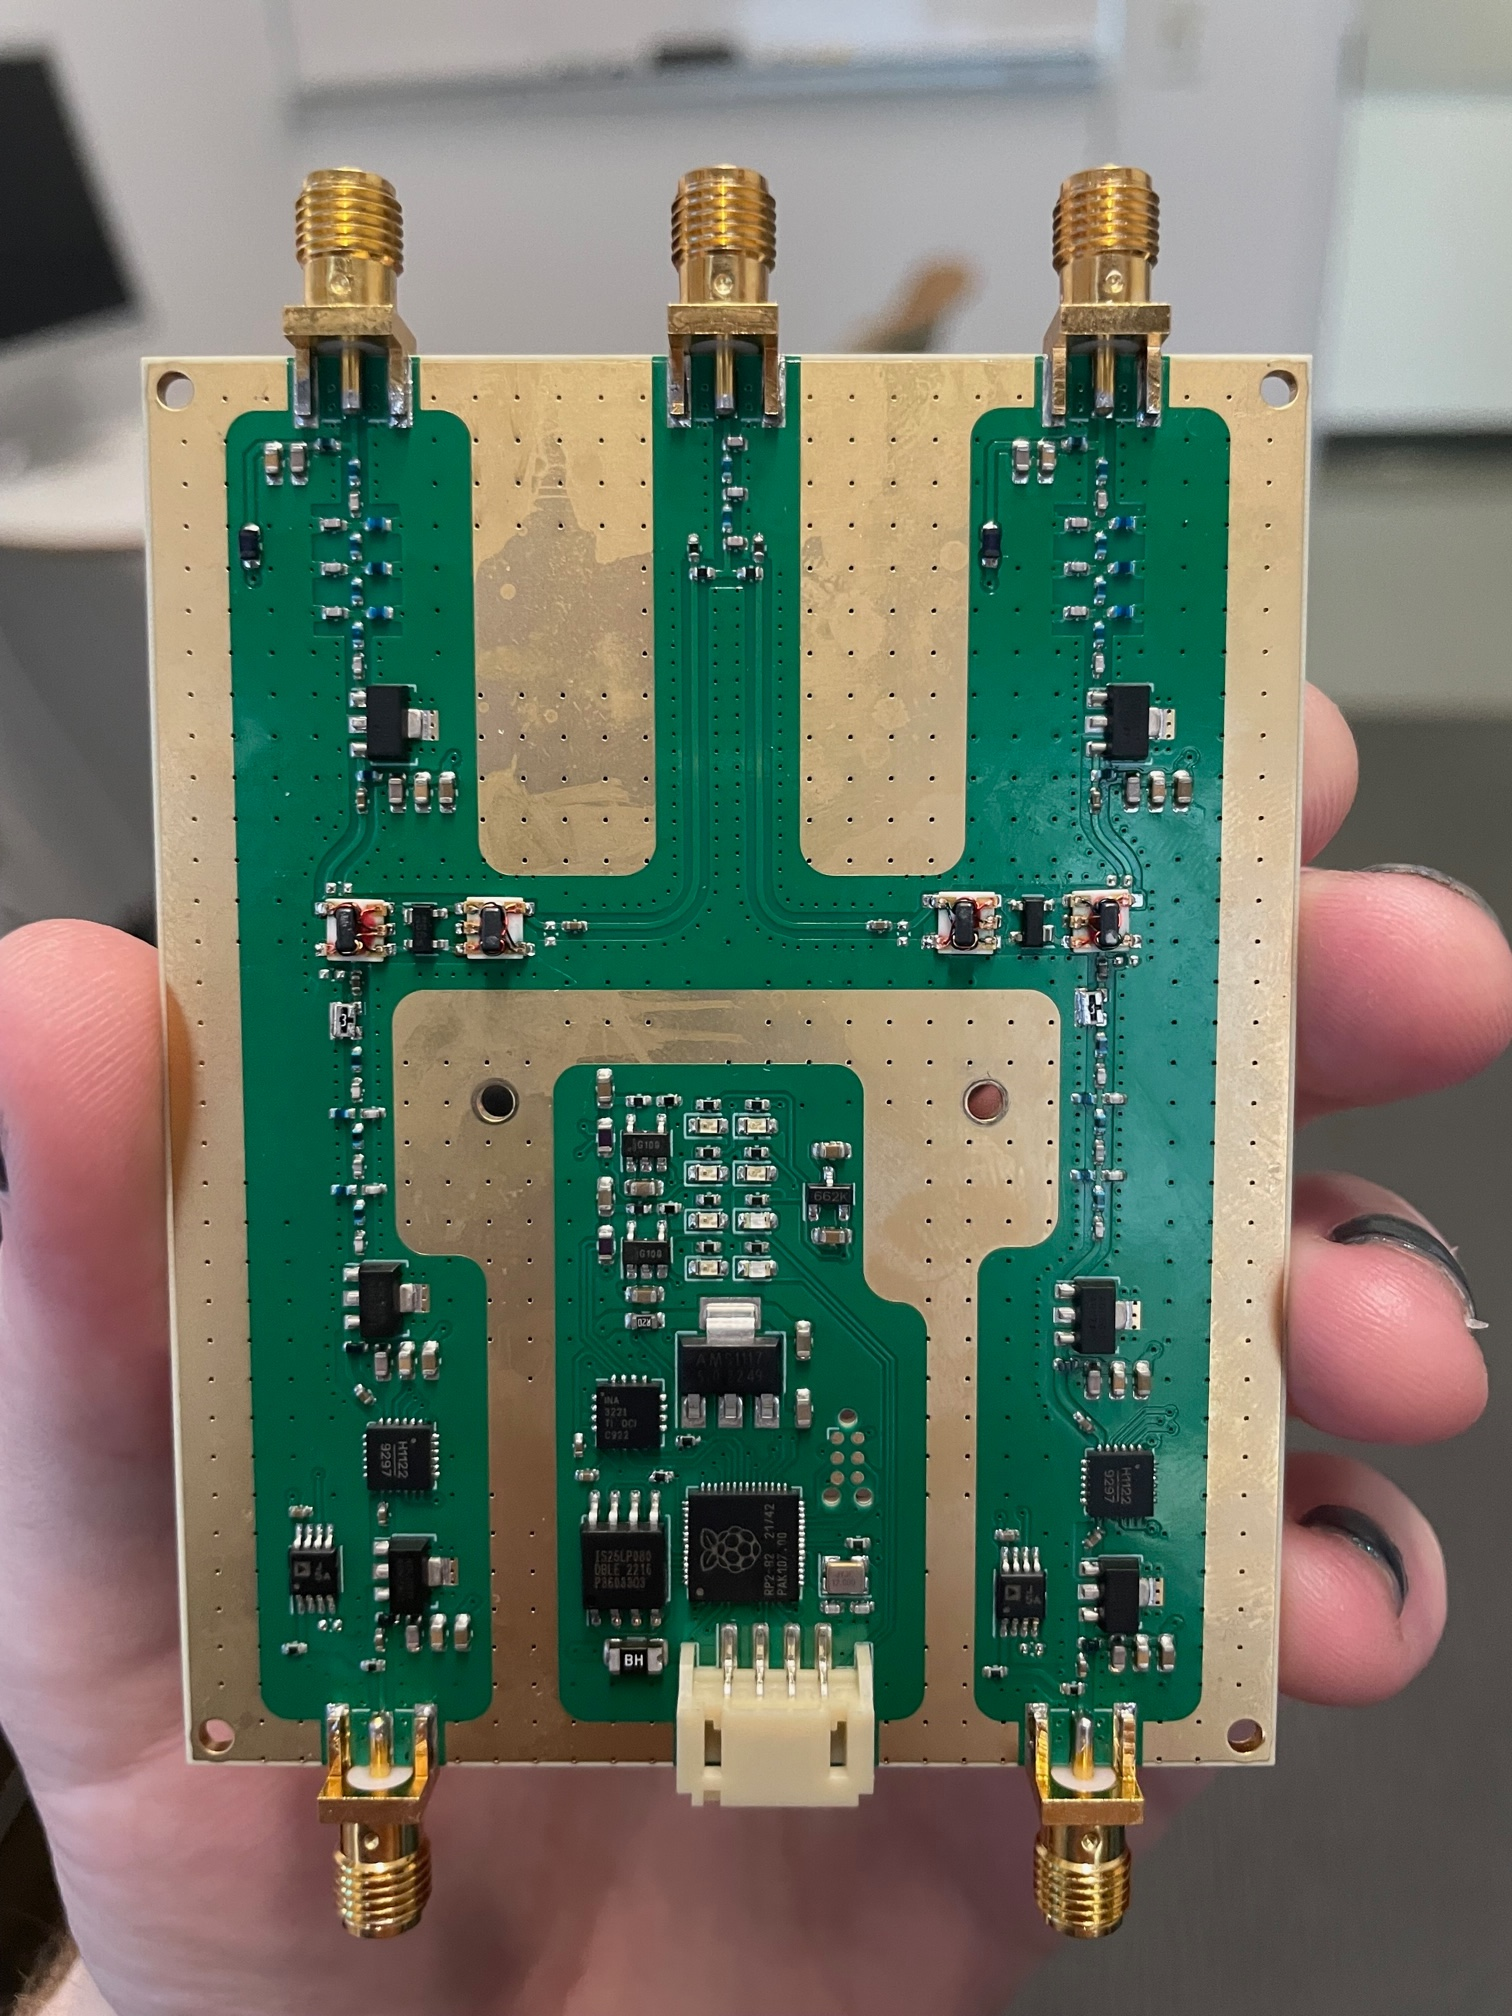
\includegraphics[width=\linewidth]{figures/FEM_PCB.jpg}
    }%
    \caption{Completed FEMs}%
    \label{fig:fem}%
\end{figure}

The heart of the analog signal processing in GReX is the frontend module (FEM).
In STARE2, the analog processing was split between electronics at the antenna and in the server room, with an RF over fiber (RFoF) link between the two sides.
Instead of RFoF, we digitize directly at the antenna, incorporating all the electronics into a single enclosure to which the antenna is bolted.
As RFoF links are typically quite nonlinear, this section of the analog signal path could limit the linear dynamic range.
To replace the RFoF circuitry, we designed the FEM to perform the frequency downconversion, filtering, and amplification needed to prepare the signal for digitization.

The FEM contains circuitry for both polarizations.
First, the signal is filtered by a $1200-1560\,\text{MHz}$ band pass filter for image frequency rejection.
Then, the signal is amplified and downconverted using a custom double-balanced mixer.
Finally, the low-frequency signal is filtered for antialiasing and amplified to drive the digitizers.

The FEM also contains digital control electronics using an RP2040 microcontroller.
This device controls the power for the LNAs connected to the FEM inputs, sets the variable attenuators, and monitors temperatures and average RF power levels.
We wrote the firmware in the Rust programming language using the RTIC~\cite{erikssonRealtimeMassesStep2013} framework for real-time task-based concurrency.
Monitoring and control is performed via a simple serial connection.

The FEM enclosure is custom machined with channels that isolate the two polarizations from the digital electronics.
This enclosure also acts as the heat sink, as it is bolted directly to a large aluminum panel inside the box.
The FEMs were fully factory-assembled, with the total per-unit cost under \$200 USD.
The completed FEM enclosure and PCB is shown in \autoref{fig:fem}.
The conversion gain of the FEM is shown in \autoref{fig:fem_bandpass}.

\begin{figure}[t!]
    \centering
    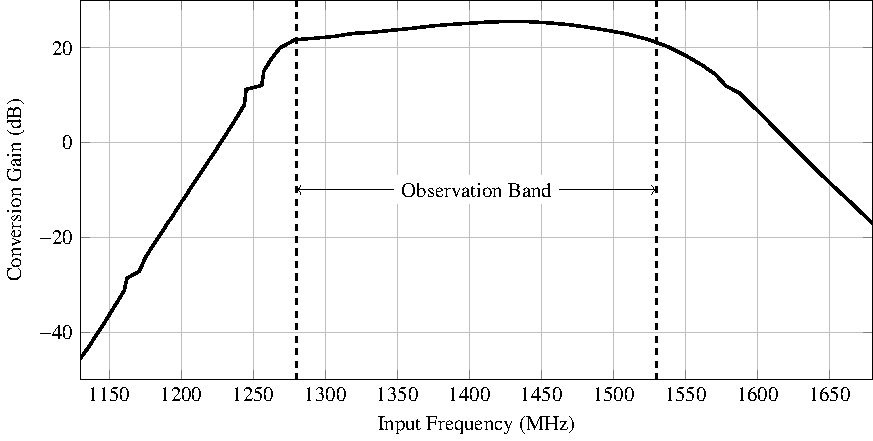
\includegraphics[width=\linewidth]{figures/fem_bandpass.pdf}
    \caption[Measured conversion gain of the FEM]{Measured conversion gain of the FEM. Total system gain adds $40\,\text{dB}$ from the LNA and $15\,\text{dB}$ from ADC preamplifiers}
    \label{fig:fem_bandpass}
\end{figure}

\subsection{The Box}

\begin{figure}[ht!]
    \centering
    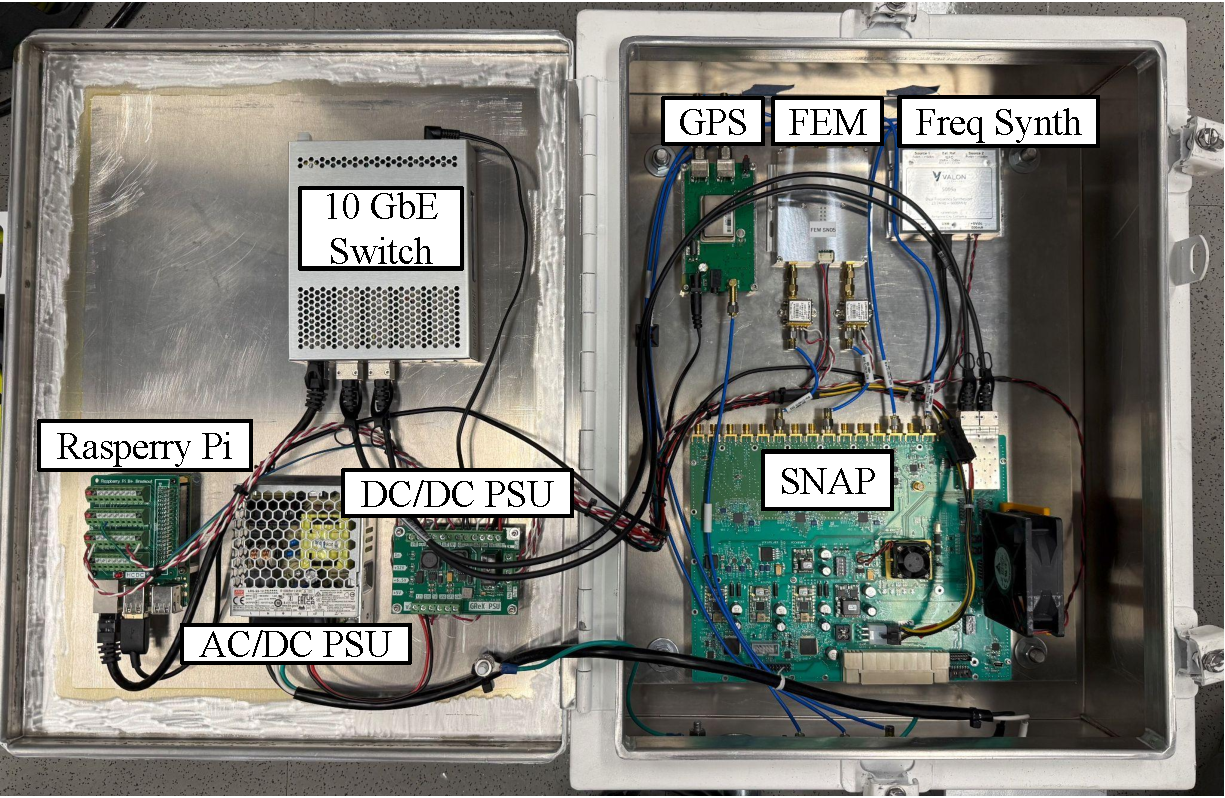
\includegraphics[width=\linewidth]{figures/box_inside.pdf}
    \caption[Inside a GReX box]{Inside a GReX box. The left panel contains the 10 GbE switch, two power supply units (PSU), and the Raspberry Pi for monitor and control. The right half contains the GPS timing receiver, frontend module (FEM), frequency synthesizer, and SNAP digitizer.}
    \label{fig:box_inside}
\end{figure}

The constructed telescope is contained in a single weatherproof aluminum box.
This box contains a GPS timing system and oscillators, the FEM, the FPGA digitizer, power supplies, a 10G Ethernet switch, and a Raspberry Pi for monitor and control.
As the box we chose had no inherent RFI shielding, we added an aftermarket weatherproof RFI gasket.
The FEM, synthesizer, GPS receiver, and FPGA digitizer are bolted to a subpanel inside the box.
The two polarization connections and GPS antenna are connected via feedthrough connectors on the bottom of the box.
The optical fiber is routed through a waveguide cutoff pipe that is attached to the bottom of the box, where it is internally terminated to a 10G SFP+ connector, attached to the Ethernet switch.
The box has mounting points on the outside for a stand or pipe and boltholes to mount the antenna.
The antenna is bolted on the top of the box with weatherproofing gasket material to prevent any water leaks.

Installation of the box is indented to be simple, requiring two single-mode fibers for the Ethernet connection and mains AC power.
Upon receiving a box, the operator needs to bolt the antenna to the top with the weatherproofing compound, then mount it to an appropriate place with a clear view of the sky.
Ideally, the antenna should be covered with RF-transparent material for weatherproofing, but we found any piece of low-loss material such as a plastic trash can to be sufficient.
A picture of an assembled box is shown in \autoref{fig:box_inside}.
